\documentclass{article}
\usepackage[utf8]{inputenc}
\usepackage{array}
\usepackage{float}
\usepackage{graphics}
\usepackage{graphicx}
\usepackage{amsmath}
\usepackage{amssymb}
\usepackage{mathrsfs}

 \setlength{\parindent}{10px}


\title{\textbf{Un algoritmo de dos fases para reconocer actividades humanas en el contexto de la industria 4.0 y procesos impulsados por el ser humano}}

\author{Borja Bordel$^1$, Ramón Alcarria$^1$, Diego Sánchez-de-Rivera$^1$ \\
\\
$^1$ Universidad Politécnica de Madrid,\\
Madrid, España\\
bbordel@dit.upm.es, ramon.alcarria@upm.es, diegosanchez@dit.upm.es}

\date{}

\begin{document}

\pagestyle{empty}

\maketitle

\thispagestyle{empty}

\subsection*{}
\textbf{Abstracto.} Futuros sistemas industriales, una revolución conocida como Industria 4.0, son concebidos para integrar personas en el mundo cibernético como prosumidores (proveedores de servicios y consumidores). En este contexto, los procesos impulsados por el ser humano aparecen como una realidad esencial y como herramientas para crear bucles de feedback entre el subsistema social (personas) y el subsistema cibernético (componentes tecnológicos) que son requeridos. Aunque se han propuesto diferentes herramientas, hoy en día las técnicas de reconocimiento de patrones son las mas prometedoras. Sin embargo, estas soluciones presentan algunos problemas pendientes importantes. Por ejemplo, dependen del hardware seleccionado para para adquirir información de e usuarios; o presentan un límite en la precisión del proceso de reconocimiento. Para abordar esta situación, en este paper está propuesto un algoritmo de dos fases para integrar personas en el sistema de la industria 4.0 y procesos impulsados por el ser humano. El algoritmo define acciones complejas como composiciones de movimientos simples. Las acciones complejas están reconocidas como Modelos Ocultos de Markov, y los movimientos simples están identificados usando Deformaciones Dinámicas en el Tiempo. De esa manera, solo los movimientos dependen de los dispositivos de hardware contratados para obtener información, y la precisión del reconocimiento de acciones complejas se ve enormemente incrementada. Una validación experimental real también es llevada a cabo para evaluar y comparar el rendimiento de la solución propuesta. \\
\\
\textbf{Palabras clave:} Industria 4.0, reconocimiento de patrones, Deformación Dinámica del Tiempo, Inteligencia artificial, Modelos ocultos de Markov

\section{Introducción}

Industria 4.0 [1] se refiere al uso de sistemas Ciber-Físicos (uniones de procesos físicos y cibernéticos) [2] como el principal componente digital en futuras soluciones digitales, principalmente (pero no solamente) en escenarios industriales. Generalmente, la digitalización ha causado, al final, el recambio de mecanismos de trabajo tradicionales por nuevos medios digitales. Por ejemplo, trabajadores en cadenas de montaje fueron sustituidos por robots durante la tercera revolución industrial.
\\
Sin embargo. Algunas aplicaciones industriales no pueden estar basadas en soluciones tecnológicas, el trabajo humano es todavía esencial [3]. Productos hechos a mano son un ejemplo de aplicaciones donde la presencia de trabajo manual es esencial. Estos sectores industriales, en cualquier caso, deben también ser integrados en la cuarta revolución industrial. De la unión de sistemas Ciber-Físicos (CPS) y humanos actuando como proveedores de servicio (trabajos activos), CPS humanizados surgen [4]. En estos nuevos sistemas, están permitidos los procesos impulsados por el ser humano [5]; e.g. procesos que son conocidos, ejecutados y organizados por personas (aunque quizás estén siendo vigilados por mecanismos digitales).
\\
Para crear una integración real entre personas y tecnología, y trasladar el proceso de ejecución del subsistema social (humanos) al mundo cibernético (componentes de hardware y software), son necesarias técnicas de extracción de información. Muchos diferentes enfoques y soluciones han sido citados durante los últimos años, pero hoy en día las técnicas de reconocimiento de patrones son las más prometedoras.
\\
El uso de inteligencia artificial, modelos estadísticos y otras herramientas similares han permitido increíble y real desarrollo de soluciones de reconocimiento de patrones, pero algunos retos siguen en el aire.
\\
En primer lugar, las habilidades de reconocimiento de patrones dependen del dispositivo de hardware subyacente para la captura de información. La estructura y procesos de aprendizaje cambian si (por ejemplo) en lugar de acelerómetros consideramos sensores de infrarrojo. Esto es muy problemático ya que la tecnología del hardware evoluciona mucho más rápido que las soluciones de software.
\\
Y, en segundo lugar, hay un límite para la precisión del proceso de reconocimiento. De hecho, mientras los actos humanos se vuelven más complicados, más variables y modelos complejos se requieren para reconocerlos. Este enfoque genera grandes problemas de optimización cuyo error residual es tan alto como el incremento del numero de variables; lo cual causa un declive en la tasa de reconocimiento [6]. En conclusión, las matemáticas (no el software, aunque depende de la implementación) fuerza una gran precisión para el proceso de reconocimiento de patrones dadas las acciones a estudiar. Para evitar esta situación, se debería considerar un menor número de variables, pero esto también reduce la complejidad de las acciones que puedan ser analizadas; una solución la cual no es aceptable en escenarios industriales donde las actividades de producción complejas son desarrolladas.
\\
Por lo tanto, el objetivo de este paper es describir un nuevo algoritmo de reconocimiento de patrones que guíe estos dos problemas básicos. El mecanismo propuesto define acciones como una composición de movimientos simples. Estos son reconocidos usando técnicas de deformaciones dinámicas en el tiempo (DTW) [7]. Este proceso depende del hardware seleccionado para la colecta de información; pero el DTW  es muy flexible y actualizando el repositorio del patrón es suficiente para configurar el algoritmo entero. Después, las acciones complejas son reconocidas como combinaciones de movimientos simples a través de Modelos Ocultos de Markov (HMM) [8]. Estos modelos son totalmente independientes de la tecnología hardware, ya que solo cuentan con acciones simples. Este enfoque de dos fases también reduce la complejidad de los modelos, incrementando la precisión y la tasa de éxito en el proceso de reconocimiento.
\\
El resto del paper se organiza de la siguiente manera: La sección 2 describe el estado del arte del reconocimiento de patrones para actividades humanas; La sección 3 describe la solución propuesta, incluyendo las dos fases definidas; La sección 4 presenta una validación experimental usando un escenario real y usuarios finales; y la sección 5 finaliza el paper.

\section{Estado del arte en el reconoccimiento de patrones}

Distintas técnicas de reconocimiento de patrones para actividades humanas han sido reportadas. Sin embargo, la propuesta más común puede clasificarse en cinco categorías [9]: (i) Modelos ocultos de Markov; (ii) el campo aleatorio condicional de cadena de salto; (iii) Patrones Emergentes; (iv) el Campo Aleatorio Condicional; y (v) clasificadores Bayesianos.

De hecho, la mayoría de los autores proponen el uso de Modelos Ocultos de Markov (HMM) para modelar las actividades humanas. HMM permite modelar acciones como cadenas de Markov [10][11]. Básicamente, HMM genera estados ocultos a partir de datos observables. En particular, el objetivo final de esta técnica es construir la secuencia de estados ocultos que encaje con una determinada secuencia de datos. Para finalmente definir el modelo, HMM debe deducir de los datos los parámetros del modelo de manera fiable. La figura 1 muestra una representación esquemática de cómo HMM trabaja. Cuando las actividades humanas son reconocidas, las acciones que componen las actividades son los estados ocultos, y las salidas de los sensores son los datos en estudio. HMM, además, permite el uso de técnicas de entrenamiento considerando el conocimiento previo sobre el modelo. Este entrenamiento a veces es esencial para “inducir” todas las posibles secuencias de datos requeridas para calcular el HMM. Finalmente, es muy importante tener en cuenta que los HMM aislados simples se pueden combinar para crear modelos más grandes y complejos.
\begin{figure}[H]
  \centering
  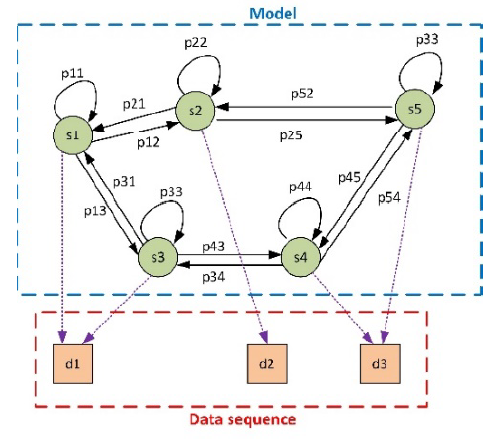
\includegraphics[scale=0.65]{foto1.png}
  \caption{Representación gráfica de una HMM}
\end{figure}

Los HMM, sin embargo, son inútiles para modelar ciertas actividades concurrentes, por lo que otros autores han reportado una nueva técnica denominada Conditional Random Field (CRF). Los CRF son empleados para modelar aquellas actividades que presentan acciones concurrentes o, en general, múltiples acciones que interactúan [12][13]. Además, HMM requiere un gran esfuerzo de entrenamiento para descubrir todos los posibles estados ocultos. Para resolver estos problemas, el campo aleatorio condicional (CRF) emplea probabilidades condicionales en lugar de distribuciones de probabilidad conjunta. De esa manera, las actividades cuyas acciones se desarrollan en cualquier orden pueden ser fácilmente moldeadas. A diferencia de las cadenas en HMM, CRF emplea gráficos acíclicos y permite la integración de estados ocultos condicionales (estados que dependen de observaciones pasadas y/o futuras).

Los CRF, por otro lado, siguen siendo inútiles para modelar ciertos comportamientos, por lo que algunas propuestas generalizan este concepto y proponen el Skip Chain Conditional Random Field (omitir campo aleatorio condicional de cadena)(SCCRF). SCCRF es una técnica de reconocimiento de patrones, más general que CRF, que permite modelar actividades que no son una secuencia de acciones en la naturaleza [14]. Esta técnica trata de capturar dependencias de largo alcance (cadena de salto); y puede entenderse como el producto de diferentes cadenas lineales. Sin embargo, al calcular este producto es bastante intenso y complicado, por lo que esta técnica suele ser demasiado costosa desde el punto de vista computacional para implementarla en pequeños sistemas integrados.

Otras propuestas emplean técnicas de descripción de mayor nivel como Emerging Patterns (Patrones emergentes)(EP). Para la mayoría de los autores, EP es una técnica que describe actividades como vectores de parámetros y sus valores correspondientes (ubicación, objeto, etc.) [15]. Utilizando distancias entre vectores es posible calcular y reconocer acciones desarrolladas por personas. Finalmente, otros autores han empleado con éxito técnicas secundarias como los clasificadores Bayesianos [16], que identifican actividades haciendo una correspondencia entre las actividades humanas y las salidas más probables de los sensores mientras se realizan estas acciones, considerando que todos los sensores son independientes. Los árboles de decisión [17], las extensiones HMM [18] y otras tecnologías similares también se han estudiado en la literatura, aunque estas propuestas son escasas.

Entre todas las teccnologías descritas, HMM no es la más poderosa. Sin embargo encaja a la perfección con la Industria 4.0, donde las actuaciones son muy complejas pero muy estructuradas y ordenadas (según protocolos de empresa, políticas de eficiencia, etc). Ademas, se requiere una retroalimentación rápida (a veces incluso en tiempo real) para garantizar que los procesos impulsados por humanos funcionen correctamente antes de que ocurra una falla crítica global. Por lo tanto, las soluciones computacionalmente costosas son un enfoque válido, y estamos seleccionando HMM como tecnología de base prirncipal. Para preservar su carácter liviano y, al mismo tiempo, poder modelar actividades complejas, introducimos un esquema de reconocimiento de dos fases que permite dividir acciones complejas en dos pasos más simples.


\section{Un algoritmo de reconocimiento de patrones de dos fases}

Con el fin de (i) independizar el proceso de reconocimiento de patrones de los dispositivos de hardware empleados para capturar información, (ii) permitir el reconocimiento de acciones complejas y (iii) preservar el carácter ligero de los modelos seleccionados, la solución propuesta presenta una arquitectura con tres capas(fases) diferentes (ver Figura 2). \\
%figura 2
\begin{figure}[H]
  \centering
  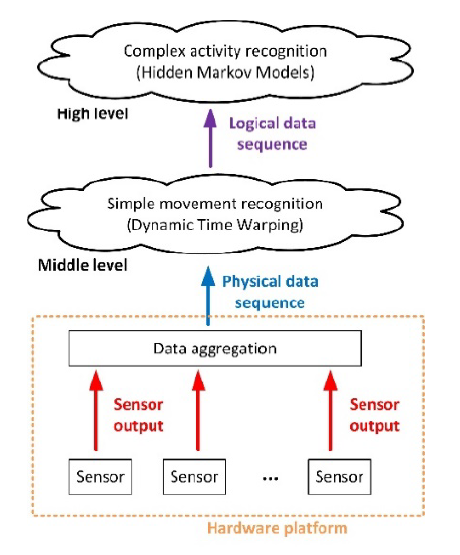
\includegraphics[scale=0.65]{foto2.png}
  \caption{
Arquitectura de la solución de reconocimiento de patrones propuesta}
\end{figure}

La capa más baja incluye la plataforma de hardware. Los dispositivos de monitoreo como acelerómetros, teléfonos, sensores infrarrojos, etiquetas RFID, etc., se implementan para capturar información sobre el comportamiento de las personas. Las salidas de estos dispositivos crean secuencias de datos físicos cuyo formato, rango dinámico, etc., dependen totalmente de las tecnologías de hardware seleccionadas.

Estas secuencias de datos físicos luego se procesan en la capa intermedia utilizando técnicas DTW. Como resultado, para cada secuencia de datos físicos, se reconoce un movimiento o acción simple. Estas acciones simples se representan mediante un formato de datos binarios para hacer la solución lo más ligera posible. El software en este nivel debe modificarse cada vez que se actualiza la plataforma de hardware, pero las tecnologías DTW no requieren un proceso de actualización complejo, y actualizar el repositorio de patrones es suficiente para configurar el algoritmo en este nivel.

Despues, los movimientos simples reconocidos se agrupan para crear secuencias de datos lógicos. Estas secuencias alimentan un sistema de reconocimiento de patrones de alto nivel basado en Modelos Ocultos de Markov. En este nivel, los componentes de software requieren un proceso de entrenamiento complejo, pero la capa intermedia hace que la plataforma de hardware y los modelos de alto nivel sean totalmente independientes. Por lo tanto, cualquier cambio en la plataforma de hardware no provoca una actualización en el HMM, la cual sería extremadamente cara desde el punto de vista computacional. Mediante el análisis de la secuencia de movimientos simples, se reconocen acciones complejas. La siguiente subsección describe detalladamente las dos fases de reconocimiento de patrones propuestas.
\\
\subsection{Reconocimiento de movimiento simple: deformación dinámica del tiempo}
Para reconocer gestos o movimientos simples, se selecciona una solución Dynamic Time Warping. Las tecnologías DTW cumplen con los requisitos de los componentes de software de nivel medio, ya que se adaptan muy fácilmente a las características de la plataforma de hardware subyacente y son bastante rápidas y eficientes (por lo que los pequeños dispositivos integrados pueden implementarlas).

En nuestra solución, el comportamiento humano se controla a través de una familia de sensores $\mathscr{S}$ , que contiene $N_s$ componentes (1).



Las salidas de estos sensores se muestran periódicamente cada $T_s$ segundos; obteniendo para cada instante de tiempo, $\mathscr{t}$, un vector de $N_s$ valores (cada valor de cada sensor). Este vector $Y_t$ se llama “una muestra multidimensional”. 

Despues, un movimiento simple $\mathscr{Y}$ tendrá una duración de $T_m$ segundos y será descrito por la secuencia temporal de $N_m$ muestras multidimensionales recolectadas durante este tiempo (3). Para reconocer posteriormente los movimientos, se crea un repositorio de patrones $\mathscr{R}$ que contiene las secuencias temporales correspondientes a cada una de las $\mathscr{K}$ acciones simples a reconocer(4).

En general, las personas realizan movimientos similares pero de manera diferente. Así, las transiciones pueden ser más lentas o más rápidas, se pueden agregar o quitar algunas acciones elementales, etc. Por lo tanto, dada una secuencia $\mathscr{X}$ con $N_x$  muestras, representando un movimiento a reconocer, se debe ubicar el patrón $R_i$  $\in$  $\mathscr{R}$ más cerca de $\mathscr{X}$; entonces $R_i$ se reconoce como la acción realizada. Para ello se define una función distancia (5). Esta función de distancia se puede aplicar para calcular una matriz de costes, requerida ya que las muestras generalmente no tienen la misma longitud ni están alineadas (6).

En los sensores posicionales (acelerómetros, dispositivos infrarrojos, etc.) la función de distancia se aplica directamente a las salidas de los sensores (a diferencia de, por ejemplo, los micrófonos cuyas salidas deben evaluarse en el dominio de la potencia). Aunque se pueden emplear otras funciones de distancia (la divergencia simétrica de Kullback-Leibler o la distancia de Manhattan), para este primer trabajo estamos empleando la distancia euclidiana estándar (7)

Luego, se define una ruta de deformación $\mathscr{p}$ = ($\mathscr{p_1}$ , $\mathscr{p_2}$ ,..., $\mathscr{p_l}$) como una secuencia de pares ($\mathscr{n_l}$ , $\mathscr{m_l}$) con ($\mathscr{n_l}$ , $\mathscr{m_l}$) $\in$ [1,$\mathscr{N_x}$] × [1,$\mathscr{N_m}$] y $\mathscr{l}$ $\in$ [1,$\mathscr{L}$], satisfaciendo tres condiciones: (i) la condición de contorno, es decir, $\mathscr{p_1}$ = [1,1] y $\mathscr{p_l}$ = [$\mathscr{N_x}$, $\mathscr{N_m}$]; (ii) la condición de monotonicidad, es decir, $\mathscr{n_1}$ $\leq$ $\mathscr{n_2}$ $\ldots$ $\leq$ $\mathscr{n_l}$ y $\mathscr{m_1}$ $\leq$ $\mathscr{m_2}$ $\ldots$ $\leq$ $\mathscr{m_l}$ ; y (iii) la condición del tamaño del paso, es decir, $\mathscr{p_l}$-$\mathscr{p_{l-1}}$ $\in$ $\left\lbrace(1,0), (0,1), (1,1)\right\rbrace$ con $\mathscr{l}$ $\in$ [1, $\mathscr{L-1}$].

Finalmente, el movimiento simple reconocido de la secuencia de datos $\mathscr{X}$ es aquel cuyo patrón $\mathscr{R_i}$ tiene la distancia más pequeña (es el más cercano) a $\mathscr{X}$. El uso de esta definición es tolerante a las variaciones de velocidad en la ejecución del movimiento, a la introducción de nuevos microgestos, etc. Además, como se puede observar, cuando se despliega una tecnología de hardware diferente, basta con actualizar el repositorio de patrones $\mathcal{R}$ para reconfigurar toda la solución de reconocimiento de patrones (ya que no se requiere capacitación).

\subsection{Reconocimiento de acciones complejas: modelos ocultos de Markov}
El mecanismo propuesto anteriormente es muy útil para reconocer acciones simples, pero las actividades complejas requieren una gran cantidad de variables y requieren mucho más tiempo. Por lo tanto, DTW tiende a ser impreciso y se requieren modelos probabilísticos. Entre todos los modelos existentes, HMM es el más adecuado para escenarios industriales y procesos impulsados ($\bullet$)por humanos.

% parrafos que faltan por las formulas

Luego, el HMM para cada actividad compleja $\mathscr{\lambda_i}$ a reconocer se describe mediante estos tres elementos anteriores (13).

Además, se hacen dos suposiciones: (i) la suposición de Markov (14) que muestra que cualquier estado sólo depende del anterior; y (ii) el supuesto de independencia (15) que establece que cualquier secuencia de observación depende únicamente del estado actual, no de estados u observaciones anteriores.

Para evaluar el modelo y reconocer la actividad que realizan los usuarios, en este artículo estamos utilizando un enfoque tradicional (16). Aunque se ha demostrado que los algoritmos directos son más eficientes, para este trabajo inicial estamos implementando directamente la expresión de evaluación en su forma tradicional.

El proceso de aprendizaje también se implementó en su forma más sencilla. Se emplearon definiciones estadísticas para matriz transitoria, matriz de observación y matriz de probabilidad inicial. En particular, se empleó la definición de probabilidad de Laplace para estimar estas tres matrices a partir de estadísticas sobre las actividades en estudio (17-19). El operador ($\bullet$) indica el número de veces que ocurre un evento

% Punto 4
\section{Validación experimental: Implementación y resultados}

Con el fin de evaluar la actuación de la solución propuesta, se ha diseñado una validación experimental para poder llevarla a cabo. Un escenario industrial fue emulado en unas habitaciones de la Universidad Politécnica de Madrid. Este escenario representa una compañía tradicional que fabrica productos hechos a mano. En especial unos fabricantes de PCI ( placas de circuito impreso) fueron emulados.

Con el fin de conseguir información sobre el comportamiento de las personas, a los participantes se les entregó un guante cibernético, el cual incluía acelerómetros y un lector de RFID [19]. Los objetos de alrededor de los escenarios fueron identificados con una etiqueta RFID, con lo que el hardware propuesto es capaz de identificar la posición de la mano (gestos) y los objetos con los que interactúa.

Una lista de 12 diferentes actividades complejas fueron definidas y reconocidas usando la tecnología propuesta. La tabla 1 describe esas 12 actividades incluyendo una descripción corta sobre ellas.

\begin{center}
\textbf{Tabla 1}. Descripción de las actividades complejas
\end{center}



\begin{table}[H]
\begin{flushleft}
\begin{tabular}{ | m{5cm} | m{6cm} | }
\hline \textbf{Actividad} & \textbf{Descripción} \\ \hline
Dibujar los caminos del circuito & El circuito a imprimir es diseñado usando un programa de software específico para PC. \\ \hline
Imprimir el circuito diseñado usando un trazador gráfico & El circuito es impreso usando una lamina de plástico y una impresora especial llamada trazadora gráfica. \\ \hline
Limpiar el laminado de tableros con el lado de cobre & Todo el polvo y las partículas se remueven del laminado de cobre usando un producto especial. \\ \hline
Copiar el diseño del circuito en tableros de cobre & El diseño del circuito que esta en las hojas de plástico se copia en el laminado de cobre usando unos rayos de luz UV. \\ \hline
Introducir los tableros en una piscina acida & La tabla se introduce en un baño de acido para retirar todo el cobre sobrante. \\ \hline
Lavar el cobre usando un baño de disolvente & Después del baño de ácido, la superficie de cobre restante si lava con un baño de disolvente. \\ \hline
Inspección Óptica & La capa de alineación se comprueba usando un laser. \\ \hline
Unir las capas exteriores con el sustrato & La capa final y la exterior del tablero se unen usando pegamento. \\ \hline
Unir el tablero & La unión de se hace en una mesa de acero pesado con abrazaderas metálicas. \\ \hline
Taladrar los agujeros necesarios & Los agujeros para componentes de perforan en el tablero. \\ \hline
Enchapado & El tablero se termina en un horno \\ \hline
\end{tabular}
\end{flushleft}
\end{table}

En el experimento estuvieron envueltas dieciocho (18) personas. Se les pidió que realizaran las actividades con un número aleatorio. Tanto el orden real como el orden en que las actividades se reconocen fueron almacenadas por un proceso de software de supervisión. Se evaluó la tasa de éxito global para toda la solución, identificando (además), la misma tasa para cada una de las fases existentes.

Para evaluar la mejora obtenida en comparación con soluciones similares existentes, se emplearon las mismas secuencias de datos físicos para alimentar una solución estándar de reconocimiento de patrones basada únicamente en HMM. Utilizando un software de procesamiento de datos estadísticos, se extraen algunos resultados relevantes.

La figura 4 representa la tasa media de éxito para tres casos: a solución global, la primera fase (DTW) y la segunda fase (HMM). Además, también se incluye la tasa de éxito del enfoque tradicional basado en HMM. Como puede verse, la tecnología propuesta es, globalmente, alrededor de un 9 mejor que las técnicas tradicionales de reconocimiento de patrones basadas exclusivamente en HMM. Además la primera fase (basada en DTW) es alrededor de un 20 peor que la segunda fase (HMM), lo que es significativo ya que la técnicas de deformación dinámica del tiempo son más débiles de forma predeterminada.

\begin{figure}[H]
  \centering
  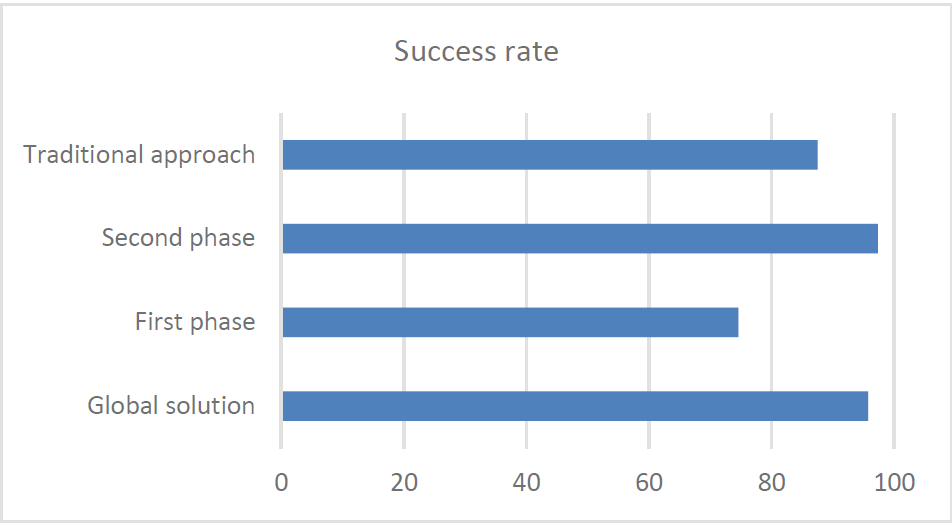
\includegraphics[scale=0.65]{grafica.png}
  \caption{Tasa media de éxito de la solución propuesta}
\end{figure}

\section{Conclusiones y trabajos futuros}

En este paper presentamos un nuevo algoritmo de reconocimiento de patrones para integrar a personas en los sistemas de la  Industria 4.0 y en procesos impulsados por humanos. El algoritmo define actividades complejas como composiciones de movimientos. Las actividades complejas se reconocen usando los modelos de Cadenas de Markov y los movimientos simples usando Dynamic Time Warping. Para poder implementar este algoritmo en pequeños dispositivos integrados, seleccionamos ligeras configuraciones. También se lleva a cabo una validación experimental, y los resultados muestran una mejora global en la tasa de éxito en torno al 9%.
\\
Los futuros trabajos necesitaran una metodología más compleja para el procesado de datos, y la comparación de diferentes configuraciones del algoritmo propuesto serán evaluadas. Además, el propósito será analizado en diferentes escenarios.
\\
\textbf{Expresiones de gratitud.}La investicacion que conllevó a estos resultados ha recibido financiación del Ministerio de Economía y Competitividad a través del proyecto SEMOLA(TEC2015-68284- R) y del Ministerio de Ciencia, Innovación y Universidades a través del proyecto VACADENA (RTC-2017-6031-2).
\\
\textbf{Referencias} 
\begin{enumerate}
\item Bordel, B., Alcarria, R., Sánchez-de-  Rivera, D.,  Robles, T. (2017, noviembre). Proteger los sistemas de la industria 4.0 contra los efectos maliciosos de los ataques ciberfísicos. En Conferencia Internacional sobre Computación Ubicua e Inteligencia Ambiental (págs. 161-171). Springer, Cham.
\item Bordel, B., Alcarria, R., Robles, T., y Martín, D. (2017). Sistemas ciberfísicos: extensión de la detección generalizada de la teoría del control al Internet de las cosas. Informática omnipresente y móvil, 40, 156-184.
	\item	Neff, W. (2017). Trabajo y conducta humana. Routledge.
	\item	Bordel, B., Alcarria, R., Martín, D., Robles, T., y de Rivera, D. S. (2017). Autoconfiguración en sistemas ciberfísicos humanizados. Revista de Inteligencia Ambiental y Computación Humanizada, 8(4), 485-496.
	\item	Bordel, B., de Rivera, D. S., Sánchez-Picot, Á., y Robles, T. (2016). Control de procesos físicos en sistemas basados en la industria 4.0: un enfoque en los sistemas ciberfísicos. En Computación Ubicua e Inteligencia Ambiental (pp. 257-262). Springer, Cham.
	\item	Pal, S. K. y Wang, P. P. (2017). Algoritmos genéticos para el reconocimiento de patrones. Prensa CRC.
	\item	Muller, M. (2007). Deformación dinámica del tiempo. Recuperación de información para música y movimiento, 69-84.
	\item	Eddy, S. R. (1996). Modelos ocultos de markov. Opinión actual en biología estructural, 6(3), 361-365.
	\item	Kim, E., Helal, S. y Cook, D. (2010). Reconocimiento de la actividad humana y descubrimiento de patrones. IEEE Pervasive Computing/IEEE Computer Society [y] IEEE Communications Society, 9(1), 48.
	\item	Li, Z., Wei, Z., Yue, Y., Wang, H., Jia, W., Burke, L. E., ... y Sun, M. (2015). Un modelo de markov oculto adaptativo para el reconocimiento de actividad basado en un dispositivo multisensor portátil. Revista de sistemas médicos, 39(5), 57.
	\item	Ordóñez, F. J., Englebienne, G., De Toledo, P., Van Kasteren, T., Sanchis, A. y Krose, B. (2014). Reconocimiento de actividad en el hogar: inferencia bayesiana para modelos ocultos de Markov. Computación generalizada de IEEE, 13(3), 67-75.
	\item	Zhan, K., Faux, S. y Ramos, F. (2015). Campos aleatorios condicionales multiescala para reconocimiento de actividad en primera persona en ancianos y pacientes discapacitados. Informática móvil y generalizada, 16, 251-267.
	\item	Liu, A. A., Nie, W. Z., Su, Y. T., Ma, L., Hao, T. y Yang, Z. X. (2015). Campos aleatorios condicionales ocultos acoplados para reconocimiento de acción humana RGB-D. Procesamiento de señales, 112, 74-82.
	\item	iu, J., Huang, M. y Zhu, X. (julio de 2010). Reconocimiento de entidades biomédicas nombradas mediante campos aleatorios condicionales de salto de cadena. En Actas del taller de 2010 sobre procesamiento biomédico del lenguaje natural (págs. 10-18). Asociación de Lingüística Computacional.
	\item	Gu, T., Wu, Z., Tao, X., Pung, H. K. y Lu, J. (marzo de 2009). epsicar: un enfoque basado en patrones emergentes para el reconocimiento de actividades secuenciales, intercaladas y concurrentes. En Computación y comunicaciones generalizadas, 2009. PerCom 2009. Conferencia internacional IEEE sobre (págs. 1-9). IEEE.
	\item	Hu, B. G. (2014). ¿Cuáles son las diferencias entre los clasificadores bayesianos y los clasificadores de información mutua?. Trans. IEEE. Red neuronal Sistema de aprendizaje, 25(2), 249-264.
	\item	Wang, X., Liu, X., Pedrycz, W. y Zhang, L. (2015). Árboles de decisión basados en reglas difusas. Reconocimiento de patrones, 48(1), 50-59.
	\item	Davis, M. H. (2018). Modelos de Markov y    optimización. Routledge.
	\item Bordel Sánchez, B., Alcarria, R., Martín,   D., y Robles, T. (2015). TF4SM: un marco            para desarrollar soluciones de trazabilidad         en pequeñas empresas manufactureras.                Sensores, 15(11), 29478-29510.
\end{enumerate}
\end{document}


\end{document}
